% Chapter 1

\chapter{Detailed guidance on the hypervisor architecture} % Main chapter title

\label{Chapter5} % For referencing the chapter elsewhere, use \ref{Chapter1} 

%----------------------------------------------------------------------------------------

% Define some commands to keep the formatting separated from the content 
%\newcommand{\keyword}[1]{\textbf{#1}}
%\newcommand{\tabhead}[1]{\textbf{#1}}
%\newcommand{\code}[1]{\texttt{#1}}
%\newcommand{\file}[1]{\texttt{\bfseries#1}}
%\newcommand{\option}[1]{\texttt{\itshape#1}}

%----------------------------------------------------------------------------------------
After the free form analysis of chapter \ref{Chapter4} it is now time to give more concrete examples on when and why the hypervisor architecture should be chosen. For this purpose several \keyword{reference projects} will be laid out and it will be discussed what makes them good or bad examples for the architecture. Afterwards some basic guidance will be given on how a specific third-party hypervisor implementation should be chosen and what metrics need to be gathered.
\section{Reference projects} \label{ref-projects}
This list of imaginary reference projects serves as a tool for the safety-critical device engineer to categorize his project's characteristics. Each project is chosen to conform with a broad category of safety-critical devices in terms of scope and criticality to make a statement about the hypervisor architectures suitability for that category.

The proposed projects are simplified and only attributes relevant to the architectural decision are examined. Metrics that can't be considered, like license cost, will not be mentioned. 

\subsection{Portable gas detector}
% https://www.elektroniknet.de/markt-technik/elektronikfertigung/perfekte-symbiose-von-oem-und-ems-151254.html
\subsubsection{Introduction}
This example project is a general, portable gas detector that measures the concentration of different gases by detecting the color change of a chemical, sensitive to the gas in question. Cartridges with clear, sealed tubes can be inserted into the device and once a measurement begins, one of the tubes is punctured and air is pumped through at a specific rate. Then the color change is observed by a \acrshort{cmos} sensor. Because the color change, pump speed and other metrics are different for every gas, information can be extracted from the cartridge via an \acrshort{nfc} tag. This tag also contains general information about the cartridge in question.
% TODO Mention device use environment

In this thought experiment the first version of this device has already been on the market for some time and now the manufacturer is looking to create the next generation. The current generation is equipped with an ARM Cortex-M4, a USB port for transmitting measurement data and an LCD display with a simplistic \acrshort{gui}. All of the software sits on top of a small \acrshort{rtos}, with the \acrshort{gui} framework also being provided by the \acrshort{rtos} developer.

In the upcoming generation the manufacturer wants to expand the device's functionality by adding Bluetooth support and a more flexible \acrshort{gui} . Furthermore, the manufacturer wants to be able to extend both the safety-critical and non-safety-critical functionality without having to release a new hardware revision. The core gas measurement code is hardware independent and already verified. Therefore, it could be included in the next generation with minimal effort, if the code's integrity can be guaranteed.
% NOTE How important is unit cost?
\subsubsection{Discussion}
% TODO I only mention SWaP but SWaP-C is probably improved. At least in terms of direct hardware cost!
The current device generation uses no separation architecture because it is not very complex and any components of lower criticality were feasible to achieve within the chosen architecture. With the upcoming generation there are now stronger initial incentives to consider the separation of software components:
\begin{enumerate}
\item There is already verified code available that the manufacturer wants to reuse with little to no modification.
\item \acrshort{gui} libraries on Linux would be a great fit for realizing a more complex \acrshort{gui} with less effort than on a typical \acrshort{rtos}. But Linux can not be feasibly verified for the safety-critical use case.
\item Both safety-critical and non-safety-critical functionality will likely be extended in the future. As established in section  \ref{safety-analysis}, granular partitions or the ability to add more can make regression testing cheaper and less error-prone.
\end{enumerate}
Additionally, the planned features do not directly impact the operators safety. The only component that can pose a threat is the \acrshort{gui} because the display could show an incorrect concentration. To mitigate this a red \acrshort{led}, controlled by the critical code, will begin blinking if the measured concentration is above the limit specified on the cartridge's \acrshort{nfc} tag. Any other failure in these components will either just prohibit retrieving data from the device for later analysis or render the device unusable. And while these effects are undesirable, the operator can recognize them and take actions to protect himself.

% NOTE References to relevant sections?
So now that the manufacturer has come to the conclusion that a separation architecture would be beneficial for the device, he needs to find one that supports his use case. For a battery powered, hand-held device \acrshort{swap} are all very important and this provides a big advantage for the hypervisor, as the \acrshort{hss} architecture compares unfavourably in regards to these criteria. Of course using the Linux \acrshort{gui} offerings would invariably lead to a stronger processor being necessary to support Linux but this would be the case for both separation architectures and for this case we will assume the manufacturer has decided that this is a worthwhile drawback for the increased graphical fidelity. 

Separating the gas measurement code from other parts of the software, at least the non verified parts, is equally doable on both architectures. However, the hypervisors support for more granular partitions makes regression testing of a software revision cheaper and can generally aid the software extendibility and maintainability.

One last benefit the hypervisor has in this scenario is established by its hardware abstraction. Any software components that are created for the next device generation will be more likely to be reusable in any future generations, with only slight or no modifications.
% TODO Maybe mention advanced safety features?
\subsubsection{Conclusion}
This project exemplifies a case where separation is becoming increasingly attractive because of growing consumer demands and processing power but where the \acrshort{hss} architecture violates the core demands of the use case. This category is likely to grow is very likely to grow in the future\cite{ITA.May2016}.

With the criticality level of the device and the specific risks involved, the hypervisor architecture's lack of support for advanced safety features and its less provable separation are no death sentence. And finally, the hypervisors malleability lends itself well to creating a future-proof design, if unit cost is not a bigger concern. 
% TODO Is there more I want to say?
\subsubsection{Implementation}
To show what the hypervisor configuration could look like for a project like the gas detector, there will be a more detailed example in this section

\subsection{Automated blood diagnostics device}
\subsubsection{Introduction}
% TODO Describe informally what the machinery does and what it consists of
This reference project is an upcoming in Vitro diagnostics device that analyzes a patients blood. Its functionalities include automatic test processing, result interpretation and data management. Blood assays include both standard blood characteristics, as well as disease screening.
The device's use environment are clinical blood labs and donation centers. It allows an operator to define and schedule automatic assays on top of displaying results on the attached operator station. The operator station consists of a monitor, a computer-mouse and a keyboard. Furthermore, the device is connected to a database of blood data for the synchronization of results.

There is a clear divide of criticality between the operator station and the components responsible for handling and analyzing the blood samples. For the operator station it is important that the assay configuration gets sent to analysis component correctly and that the test results received after an analysis are correct. Transmitting and receiving results from the database is also not critical to the patients safety.

% TODO Mention in Vitro medical standard 
The blood analysis component on the other hand is more critical. A perfect uptime is not required as a patient is not immediately dependent on the device. Instead, it is much more important that faults or incorrect measurements are discovered and communicated to an operator. Cross-contamination also needs to be avoided at all costs.

\subsubsection{Discussion}
With this device, separation is almost mandatory because the operator station contains a large low-criticality \acrshort{gui} that can be most optimally realized on a general purpose operating system, while the critical part needs to reliably control motors and react to input within a short time-frame. Traditionally this system would have been realized using the \acrshort{hss} architecture so now the question remains whether or not a hypervisor can be used effectively instead.

First of all, due to the nature of the device, perfect uptime is not required, this means that redundancy is also not essential. This works in the favor of the hypervisor, since in the \acrshort{hss} architecture only the safety-critical component could be made redundant but that option would not be available for a hypervisor because all partitions are part of one processor. 

% TODO Make smaller
% FIGURE Refine this figure
\begin{figure}
\centering
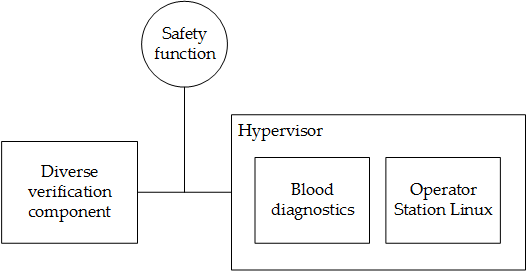
\includegraphics[scale=0.75]{Figures/blood_diagnostics_arch}
\decoRule
\caption{Example hypervisor partition setup}
\label{fig:blood_diagnostics_hv_arch}
\end{figure}

However, the system's need for fault tolerance means that some advanced fault tolerance techniques are necessary to mitigate the risks as much as possible. One way this could be achieved with a hypervisor architecture can be seen in figure \ref{fig:blood_diagnostics_hv_arch}. In this case both the safety-critical partition and the operator station partition are running on the hypervisor, with a secondary microcontroller performing the same calculations and verifying the output of the safety-critical hypervisor partition. Even though this means there are now multiple processors present, the hypervisor still provides consolidating effects. A pure \acrshort{hss} architecture would still require a minimum of three partitions for the same setup.
% FIGURE Make an architecture figure 

% NOTE The proximity things seems like bullshit. Where did I even get that from?
If we assume that the separation is adequate and all basic safety requirements can be met, there are still factors left to consider. First of all, since this is a system that deals with real-time requirements, proximity to the machinery could be valuable. But in this case \acrshort{emc} can cause significant issues. In the hypervisor setup a processor with a higher frequency would sit closer to the motors and other machinery which also themselves have \acrshort{emi}. This could easily lead to a violation of the \acrshort{emc} requirements of the regulatory body, introducing the need to add more electromagnetic shielding. 

This device can also benefit from the hypervisor's architectural improvements and easier configuration, perhaps even more so. Since it is more complex, it is also more likely that functionality can be usefully extracted into partitions, carrying the benefits explained in \ref{Chapter4}. But it is important to keep in mind that for a device with these characteristics, some of the typical hypervisor benefits are less relevant.

First of all, the hardware cost savings are not going to make a big impact on a device this complex and big. Secondly, \acrshort{swap} are also not as crucial as for the portable gas detector. The housing of this unit is already going to be at least as big as a typical wardrobe and an extra microcontroller is not going to change that. Same goes for weight. And since the device is connected to power all the time, making it as power efficient as possible is also not a primary goal.

\begin{comment}
% NOTE Did I say it is necessary in the introduction?! If not why am I arguing about his here. Bad section
One last thing that needs to be kept in mind is the typical hypervisor's current hardware restrictions. If a \acrshort{dsp} is necessary to control the device, the hypervisor could be at a disadvantage, since there is currently no \acrshort{dsp} that can host a hypervisor. But this may change in the near future (see section \ref{cortex-r52-hypervisor}).  
\end{comment}

\subsubsection{Conclusion}
This example represents a high complexity, high criticality project that can already profit from the more traditional approaches of separation but where, in a reevaluation of device architecture, the hypervisor approach might come out on top. 

Some of the hypervisor benefits are not as important as in other classes of devices but it might still be an overall better choice, if the other factors like \acrshort{emc} and safety of separation can be adequately satisfied. This example has of course been significantly simplified to construct a discussion about devices that are in this range of complexity and criticality and in a real-world example a lot more analysis will be necessary to determine whether the hypervisor is a good fit. As of 2018 this may still be a risky technical decision but with the push into hypervisors by the aviation and automotive industry, industries that manufacturer exactly this class of devices, this could evaporate within the next decade.

%----------------------------------------------------------------------------------------

\section{How to decide on a hypervisor implementation} \label{how-to-decide}
% NOTE Maybe talk about how this applies to first-party hypervisors?
This section explores the extended analysis that needs to be carried out by the manufacturer, once he is seriously considering using a third-party hypervisor. For the most part, it consists of a list of questions that need to be asked, with further explanation, if required. The categorization of the questions closely resembles the key wants established in \ref{Chapter3}.

Actually, it is conceivable that the result of this analysis reveals that no third-party hypervisors exists that can satisfy the manufacturers targets. The importance of each question is going to vary on a project by project basis and questions should be asked roughly in their order of importance. 

\subsection{Certifiability}
\paragraph{Which level of criticality does the hypervisor developer claim to be able to certify to?}
Since, this section is concerned with the concrete real-world examples, the abstract concept of criticality levels also has to be abandoned. It only makes sense to ask this question in relation to the actual regulations that the device will be certified to.

\paragraph{What deliverables and services does he offer to aid with certification?}
Usually the developer will offer documentation and test cases for the hypervisor that can be presented as evidence of safety to the regulatory bodies. But typically there is more work to do: the specifics depend on the standard but at the very least the risk of using the hypervisor needs to be evaluated and justified. Developers will also usually offer services to help with the certification of the hypervisor. Depending on the manufacturer's prowess with the regulations and the hypervisor such a service could be worthwhile.
\paragraph{Has the hypervisor successfully been used in a device that has to comply to the same regulations?}
Although, a "proven-in use" status is not enough to convince a regulatory body of a piece of software's safety it is at least evidence, that it can be done.
\paragraph{Do the claims of the developer and his documentation survive more intense scrutiny and project specific risk analysis?}
Because the hypervisor developers are clearly trying to sell a product, their claims should be met with scrutiny. This is a question that should probably be analyzed in the latter stages of the decision process.
\subsection{Cost}
The question of the hypervisor license cost has been mostly avoided in this thesis, since it can't be answered on a general level. Now is the time to come back to it.
\paragraph{What license model is applicable and what will the license cost?}
License models tend to vary based on unit cost and rate of production.
The cost of the license is probably exclusively subject to negotiation. 
\paragraph{Is there functionality or services that cost extra? Are they desirable?}
One possibility for an extra service has already been listed; enlisting the developer to help with certification. But some, more specialized functionality may also be gated behind additional cost. Furthermore, the developers almost always offer general services surrounding the hypervisor: helping with configuration and developing more features being among them. Especially, developers of open-source hypervisors tend to sustain themselves this way.
\paragraph{What costs are associated with the operating system that will run on the hypervisor?}
This question doesn't necessarily have to do with the hypervisor developer directly, although it can. The default paravirtualized \acrshort{os} is supplied by the hypervisor developer and may incur additional costs. If the manufacturer decides to customize an operating system himself or use a fully virtualized free open-source \acrshort{os} these license costs can be avoided. 
\subsection{Dependence}
The last question in the previous section already hints at it: using a third-party hypervisor can introduce significant dependence to said third-party, especially sine the third-party also offers the \acrshort{os} running on top of the hypervisor.
\paragraph{Is the hypervisor source code available?}
\paragraph{Is it feasible for the manufacturer to modify the hypervisor on his own?}
This requires the source code to be available and legally modifiable. Such actions could include supporting additional hardware and changing or adding hypervisor functionality. If the manufacturer is planning to build expertise with the hypervisor implementation this can allow him to save costs by not enlisting the original developer to fulfill these services.

\paragraph{What paravirtualized operating systems are available and can the manufacturer feasibly add new ones?}

\paragraph{If the device has real-time requirements, can they be met with the hypervisor architecture?}
This is clearly a very difficult question to answer, before development has even begun but it still needs to be analyzed to avoid disaster.
\subsection{Additional functionality}
The core functionality the hypervisor offers has been explored in \ref{Chapter2}. This section is concerned with slightly more advanced features. Some hypervisor implementations are completely bare-bones and offer nothing beyond the features of a basic hypervisors and others offer many advanced features. This difference is likely to be reflected in the price of the respective implementations.
\paragraph{What additional functionality can the developer offer?}
Below is a list of some possible features that exist in current implementations.
% NOTE Do any items require additional explanation?
\begin{itemize}
    \item Different possible scheduling policies
    \item Health monitoring
    \item Device pass-through (Requires an \acrshort{iommu} to work effectively)
    \item Full virtualization
    \item Virtual input device support
    \item Security certifications
    \item Automatic tests during operation
    \item Virtual high resolution timers
\end{itemize}

\subsection{Impact on the development process}
\subsubsection{Tooling}
\paragraph{What tools are available for hypervisor configuration?}
The two possible categories of tools are \acrshort{cli} and \acrshort{ide} tools. A \acrshort{cli} tool may take input directly or from configuration files in a specific format. An \acrshort{ide} could instead offer a graphical representation with possible values, hints and even drag and drop configuration of some features. If done well this can greatly reduce the barrier of entry for new users, if done badly this can cloud the users understanding of the actual configuration and introduce errors.

Some regulations also require that all tools used to created safety-critical devices need to be verified and the same applies for the tools used to configure and build the hypervisor. It can be expected that an \acrshort{ide} is more expensive to verify than a \acrshort{cli} tool and while this may not impact the manufacturer directly, it may increase the cost of the hypervisor license.
\paragraph{What compilers and debuggers are supported and do they align with the project requirements?}
Compilers and potentially even debuggers need to be verified as well. This means that safety-critical device manufacturer typically use less common compilers that are already verified. If the hypervisor, for whatever reason, doesn't support that specific compiler it could incur additional cost or even render it infeasible.
\subsubsection{Debugging and tracing}
Since the hypervisor acts as a layer of abstraction between the hardware and software it has the potential to be a great aid in debugging the system. But simultaneously it could also act as a great hindrance, obfuscating issues in the business code and not providing access to partition data that would have been available without the hypervisor.
\paragraph{Does the hypervisor provide standard debugging functionality?}
There are multiple ways to achieve this and they will not be explored in detail here but the two most prominent examples are: a debugging server running on the device and a hypervisor aware \acrshort{jtag} environment. Ideally, it is possible to debug both the hypervisor and the guest operating systems independently \cite{Lauterbach.2018}. 
\paragraph{Does the hypervisor provide special debugging or tracing functionality?}
As established in section \ref{distributed-or-centralized}, the hypervisor has a unique centralized view of the system. It can therefore expose its internal events to a developer and provide high level insight into what exactly is happening inside the hypervisor.

%----------------------------------------------------------------------------------------

\section{Noteworthy implementations} \label{noteworthy-implementations}
As a contrast to the "basic safety-hypervisor" established early in the thesis, now will be given some notable 2018 implementations. Keep in mind that no claim is being made about their respective quality, it is just being pointed out what interesting and unique features or characteristics they have.
\subsection{seL4 and CAmkES} \label{seL4}
seL4 is a formally verified microkernel with a focus on security, so far it has been mostly confined to academia but some advances into realistic products have been made since \cite{fisher2012hacms}. \textquote{CAmkES (component architecture for microkernel-based embedded systems) is a software development and runtime framework for quickly and reliably building microkernel-based multiserver (operating) systems.}[source]. A system that is built with these two can also host virtual machines on some platforms. This implementation provides much more flexibility than a basic hypervisor, as it can be used to design general modular software systems. The formal verification of seL4 and CAmkES, as well as the additional verification output that can be generated automatically, can go a long way in certifying a safety-critical device.
% Link CAmkES source: https://docs.sel4.systems/CAmkES/
\subsection{SYSGO's PikeOS}
PikeOS is unique because it is a real-time operating system first and foremost with hypervisor functionality added on top. Similar to seL4 with CAmkES it can provide much more flexibility in designing the system than a hypervisor that offers only virtualized guest environments. Partitions can host \acrshort{rtos} task trees or a virtualized operating system respectively. This also eliminates the need to virtualize an \acrshort{rtos} in the first place.

Additionally, PikeOS offers a form of hierarchical scheduling which can make the scheduling of mixed criticality systems more efficient and potentially easier [source].
\subsection{OpenSynergy's COQOS MICRO SDK}
TBD
\begin{comment}
* (LynxSecure)
* Mentor (as a really small example, maybe find additional)
* PROVENVISOR (formally verified, security focus)
* GreenHills, WindRiver and maybe QNX as "expensive high-profile" hypervisors
* [...]
\end{comment}